\documentclass[]{standalone}
\usepackage{tikz}
\usetikzlibrary{shapes,arrows,calc,positioning}
\usepackage{amsmath} % for dfrac
\usepackage{comment}

% definition of basic block
\tikzset{
    block/.style = {draw, rectangle,
        minimum height=1.2cm,
        minimum width=2cm},
    input/.style = {coordinate,node distance=1cm},
    output/.style = {coordinate,node distance=1cm},
    sum/.style = {draw, circle, node distance=1cm},
}

% definition of saturation block
\tikzset{% from https://tex.stackexchange.com/questions/161075/saturation-block
  saturation block/.style={%
    draw, 
    path picture={
      % Get the width and height of the path picture node
      \pgfpointdiff{\pgfpointanchor{path picture bounding box}{north east}}%
        {\pgfpointanchor{path picture bounding box}{south west}}
      \pgfgetlastxy\x\y
      % Scale the x and y vectors so that the range
      % -1 to 1 is slightly shorter than the size of the node
      \tikzset{x=\x*.4, y=\y*.4}
      %
      % Draw annotation
      \draw (-1,0) -- (1,0) (0,-1) -- (0,1); 
      \draw (-1,-.7) -- (-.6,-.7) -- (.6,.7) -- (1,.7);
    }
  }
}

\begin{document}
	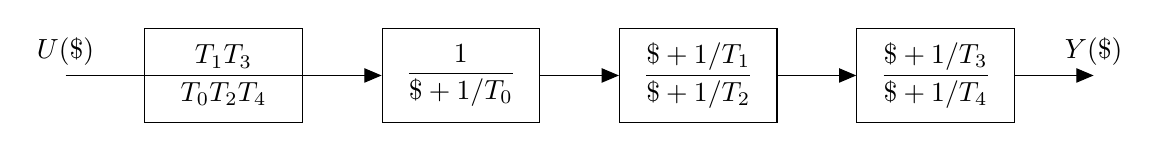
\begin{tikzpicture}[auto, node distance=1cm,>=triangle 45]

		% Lowpass
		\node [input, name=input1, ] {};
		
		\node [block, right=of input1] (gain) {$\dfrac{T_1 T_3}{T_0 T_2 T_4}$};
		
		\node [block, right=of gain] (first) {$\dfrac{1}{\$ +1/T_0}$};
		\node [block, right=of first] (second) {$\dfrac{\$ +1/T_1}{\$ +1/T_2}$};
		\node [block, right=of second] (third) {$\dfrac{\$ +1/T_3}{\$+1/ T_4}$};		
		
		\node [output, right=of third] (output1) {};
		
		
		\draw [->] (input1) node[above] {$U(\$)$} -- (first) ;
		\draw [->] (first) -- (second) ;
		\draw [->] (second) -- (third) ;
		\draw [->] (third) -- (output1) node[above] {$Y(\$)$}  ;


	
	\end{tikzpicture} 
\end{document}